\chapter{数字}
地球虽然有很多种语言,但数字大概哪里都是阿拉伯数字呢。

Arbazard毕竟是异世界,没有阿拉伯数字吧?


\emoji{l_naki} 
没有呢……阿拉伯数字。
不过作为替代,有这样的数字呢
(0~9まで)
\begin{figure}[H]
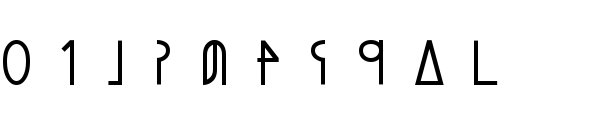
\includegraphics[width=0.7\textwidth]{ARKA/alx.jpg}
\end{figure}

\FiveStar 读法

0:yuu

1:ko 

2:ta 

3:vi 

4:val 

5:lin 

6:kis 

7:nol 

8:ten 

9:los 

\emoji{x_naki} 
0和1以外,一点看不懂(-ω-)


\emoji{a_reps} 
不过,因为是十进制的计数法,所以比较容易计数吧
顺带一说,4,5,6和7,8,9的末尾是规则的l,n,s,这可以方便记忆呢。


\emoji{l_niit} 

数数的方法和日语一样呢.10读作on.

13是on和vi的拼接,onvi。

20是ta和on的拼接,taon。


\emoji{x_knoos} 
百和千之类怎么说?


\emoji{l_asex_kal} 
百是gal,千是kot,万是sen。

例如24,345,就读做tasen valkot vigal valon lin。


\emoji{a_niit} 
和日语不同的是,一万不是kosen,就是一个sen,这个要注意
\footnote{日语里面如果是"一千"和"一百",就能省略"一",只说"千"或"百",这一点对"万"不适用.但是Arka是可以的}.


\emoji{x_niit} 
原来如此。

那么,"4个女孩子"怎么说?


\emoji{l_sena} 
是val fian。

Arka没有"人"啊"个"啊这样的量词\footnote{原文为"助数詞",译者暂时没有在网页中找到"两筐篮球"之类关于"量"的描述./*TODO*/},
只要把数放在名词前面就可以了。

顺带一说,fian val这样在名词后面九上数字也可以,这种用法,就表示序数,"第4个女孩子"


\emoji{x_sena} 
霍霍,这么方便啊.

只要换个地方就能变成号码。